% Options for packages loaded elsewhere
\PassOptionsToPackage{unicode}{hyperref}
\PassOptionsToPackage{hyphens}{url}
\PassOptionsToPackage{dvipsnames,svgnames,x11names}{xcolor}
%
\documentclass[
  ignorenonframetext,
]{beamer}
\usepackage{pgfpages}
\setbeamertemplate{caption}[numbered]
\setbeamertemplate{caption label separator}{: }
\setbeamercolor{caption name}{fg=normal text.fg}
\beamertemplatenavigationsymbolsempty
% Prevent slide breaks in the middle of a paragraph
\widowpenalties 1 10000
\raggedbottom

\usepackage{amsmath,amssymb}
\usepackage{iftex}
\ifPDFTeX
  \usepackage[T1]{fontenc}
  \usepackage[utf8]{inputenc}
  \usepackage{textcomp} % provide euro and other symbols
\else % if luatex or xetex
  \usepackage{unicode-math}
  \defaultfontfeatures{Scale=MatchLowercase}
  \defaultfontfeatures[\rmfamily]{Ligatures=TeX,Scale=1}
\fi
\usepackage{lmodern}
\usetheme[]{AnnArbor}
\usecolortheme{dolphin}
\usefonttheme{structurebold}
\ifPDFTeX\else  
    % xetex/luatex font selection
\fi
% Use upquote if available, for straight quotes in verbatim environments
\IfFileExists{upquote.sty}{\usepackage{upquote}}{}
\IfFileExists{microtype.sty}{% use microtype if available
  \usepackage[]{microtype}
  \UseMicrotypeSet[protrusion]{basicmath} % disable protrusion for tt fonts
}{}
\makeatletter
\@ifundefined{KOMAClassName}{% if non-KOMA class
  \IfFileExists{parskip.sty}{%
    \usepackage{parskip}
  }{% else
    \setlength{\parindent}{0pt}
    \setlength{\parskip}{6pt plus 2pt minus 1pt}}
}{% if KOMA class
  \KOMAoptions{parskip=half}}
\makeatother
\usepackage{xcolor}
\newif\ifbibliography
\setlength{\emergencystretch}{3em} % prevent overfull lines
\setcounter{secnumdepth}{-\maxdimen} % remove section numbering


\providecommand{\tightlist}{%
  \setlength{\itemsep}{0pt}\setlength{\parskip}{0pt}}\usepackage{longtable,booktabs,array}
\usepackage{calc} % for calculating minipage widths
\usepackage{caption}
% Make caption package work with longtable
\makeatletter
\def\fnum@table{\tablename~\thetable}
\makeatother
\usepackage{graphicx}
\makeatletter
\def\maxwidth{\ifdim\Gin@nat@width>\linewidth\linewidth\else\Gin@nat@width\fi}
\def\maxheight{\ifdim\Gin@nat@height>\textheight\textheight\else\Gin@nat@height\fi}
\makeatother
% Scale images if necessary, so that they will not overflow the page
% margins by default, and it is still possible to overwrite the defaults
% using explicit options in \includegraphics[width, height, ...]{}
\setkeys{Gin}{width=\maxwidth,height=\maxheight,keepaspectratio}
% Set default figure placement to htbp
\makeatletter
\def\fps@figure{htbp}
\makeatother
% definitions for citeproc citations
\NewDocumentCommand\citeproctext{}{}
\NewDocumentCommand\citeproc{mm}{%
  \begingroup\def\citeproctext{#2}\cite{#1}\endgroup}
\makeatletter
 % allow citations to break across lines
 \let\@cite@ofmt\@firstofone
 % avoid brackets around text for \cite:
 \def\@biblabel#1{}
 \def\@cite#1#2{{#1\if@tempswa , #2\fi}}
\makeatother
\newlength{\cslhangindent}
\setlength{\cslhangindent}{1.5em}
\newlength{\csllabelwidth}
\setlength{\csllabelwidth}{3em}
\newenvironment{CSLReferences}[2] % #1 hanging-indent, #2 entry-spacing
 {\begin{list}{}{%
  \setlength{\itemindent}{0pt}
  \setlength{\leftmargin}{0pt}
  \setlength{\parsep}{0pt}
  % turn on hanging indent if param 1 is 1
  \ifodd #1
   \setlength{\leftmargin}{\cslhangindent}
   \setlength{\itemindent}{-1\cslhangindent}
  \fi
  % set entry spacing
  \setlength{\itemsep}{#2\baselineskip}}}
 {\end{list}}
\usepackage{calc}
\newcommand{\CSLBlock}[1]{\hfill\break\parbox[t]{\linewidth}{\strut\ignorespaces#1\strut}}
\newcommand{\CSLLeftMargin}[1]{\parbox[t]{\csllabelwidth}{\strut#1\strut}}
\newcommand{\CSLRightInline}[1]{\parbox[t]{\linewidth - \csllabelwidth}{\strut#1\strut}}
\newcommand{\CSLIndent}[1]{\hspace{\cslhangindent}#1}


% logo
\titlegraphic{
\includegraphics[width=4cm]{000_logos/logo-blue-vertical}}
\logo{\ifnum\thepage>1
\includegraphics[width=0.5cm]{000_logos/logo-blue-vertical}\fi}

% UMNG: Manual de image institucional

% Colors

% Umng
\definecolor{yellow}{HTML}{fdc600}
\definecolor{red}{HTML}{ee2a24}

% Estudios a Distancia
\definecolor{blue1}{HTML}{12245b}
\definecolor{blue2}{HTML}{767ca6}
\definecolor{blue3}{HTML}{cad2ec}

% Modify items
\setbeamercolor{palette primary}{bg=blue3}
\setbeamercolor{palette tertiary}{bg=blue1}
\setbeamercolor{frametitle}{bg=yellow}

% Hyperlinks
\hypersetup{
  linkcolor=red,
  citecolor=red
}

\makeatletter
\@ifpackageloaded{caption}{}{\usepackage{caption}}
\AtBeginDocument{%
\ifdefined\contentsname
  \renewcommand*\contentsname{Table of contents}
\else
  \newcommand\contentsname{Table of contents}
\fi
\ifdefined\listfigurename
  \renewcommand*\listfigurename{List of Figures}
\else
  \newcommand\listfigurename{List of Figures}
\fi
\ifdefined\listtablename
  \renewcommand*\listtablename{List of Tables}
\else
  \newcommand\listtablename{List of Tables}
\fi
\ifdefined\figurename
  \renewcommand*\figurename{Figure}
\else
  \newcommand\figurename{Figure}
\fi
\ifdefined\tablename
  \renewcommand*\tablename{Table}
\else
  \newcommand\tablename{Table}
\fi
}
\@ifpackageloaded{float}{}{\usepackage{float}}
\floatstyle{ruled}
\@ifundefined{c@chapter}{\newfloat{codelisting}{h}{lop}}{\newfloat{codelisting}{h}{lop}[chapter]}
\floatname{codelisting}{Listing}
\newcommand*\listoflistings{\listof{codelisting}{List of Listings}}
\makeatother
\makeatletter
\makeatother
\makeatletter
\@ifpackageloaded{caption}{}{\usepackage{caption}}
\@ifpackageloaded{subcaption}{}{\usepackage{subcaption}}
\makeatother

\ifLuaTeX
\usepackage[bidi=basic]{babel}
\else
\usepackage[bidi=default]{babel}
\fi
\babelprovide[main,import]{english}
% get rid of language-specific shorthands (see #6817):
\let\LanguageShortHands\languageshorthands
\def\languageshorthands#1{}
\ifLuaTeX
  \usepackage{selnolig}  % disable illegal ligatures
\fi
\usepackage{bookmark}

\IfFileExists{xurl.sty}{\usepackage{xurl}}{} % add URL line breaks if available
\urlstyle{same} % disable monospaced font for URLs
\hypersetup{
  pdftitle={Economy and institutions},
  pdfauthor={Luis Francisco Gómez López},
  pdflang={en},
  colorlinks=true,
  linkcolor={Maroon},
  filecolor={Maroon},
  citecolor={Blue},
  urlcolor={Blue},
  pdfcreator={LaTeX via pandoc}}


\title{Economy and institutions}
\author{Luis Francisco Gómez López}
\date{2024-07-16}
\institute{FAEDIS}

\begin{document}
\frame{\titlepage}

\renewcommand*\contentsname{Table of contents}
\begin{frame}[allowframebreaks]
  \frametitle{Table of contents}
  \tableofcontents[hideallsubsections]
\end{frame}

\section{Please Read Me}\label{please-read-me}

\begin{frame}{}
\phantomsection\label{section}
\begin{itemize}
\item
  Check the message \textbf{Welcome greeting} published in the News
  Bulletin Board.
\item
  Dear student please edit your profile uploading a photo where your
  face is clearly visible.
\item
  The purpose of the virtual meetings is to answer questions and not to
  make a summary of the study material.
\item
  This presentation is based on
  (\citeproc{ref-cardenas_introduccion_2020}{Cardenas 2020, chap. 4})
\end{itemize}
\end{frame}

\section{Purpose}\label{purpose}

\begin{frame}{}
\phantomsection\label{section-1}
Analyze the role of institutions in the economy
\end{frame}

\section{Definition of institutions}\label{definition-of-institutions}

\begin{frame}{}
\phantomsection\label{section-2}
\begin{itemize}
\item
  ``Institutions are the rules of the game in a society or, more
  formally, are the humanly devised constraints that shape human
  interaction'' (\citeproc{ref-north_institutions_1990}{Douglass C.
  North 1990, 3})
\item
  Institutions can be informal or formal
  (\citeproc{ref-north_institutions_1991}{Douglass C. North 1991})

  \begin{itemize}
  \item
    \textbf{Informal}: sanctions, taboos, customs, traditions, and codes
    of conduct
  \item
    \textbf{Formal}: constitutions, laws, property right
  \end{itemize}
\end{itemize}
\end{frame}

\section{Measuring formal
institutions}\label{measuring-formal-institutions}

\begin{frame}{}
\phantomsection\label{section-3}
\begin{itemize}
\item
  Governance

  \begin{itemize}
  \item
    Set of traditions and institutions by which authority in a country
    is exercised where it includes
    (\citeproc{ref-kaufmann_worldwide_2011}{Kaufmann, Kraay, and
    Mastruzzi 2011, 222}):

    \begin{itemize}
    \tightlist
    \item
      The process by which governments are selected, monitored and
      replaced
    \item
      The capacity of the government to effectively formulate and
      implement sound policies
    \item
      The respect of citizens and the state for the institutions that
      govern economic and social interactions among them
    \end{itemize}
  \end{itemize}
\end{itemize}
\end{frame}

\begin{frame}{}
\phantomsection\label{section-4}
\begin{figure}

\centering{

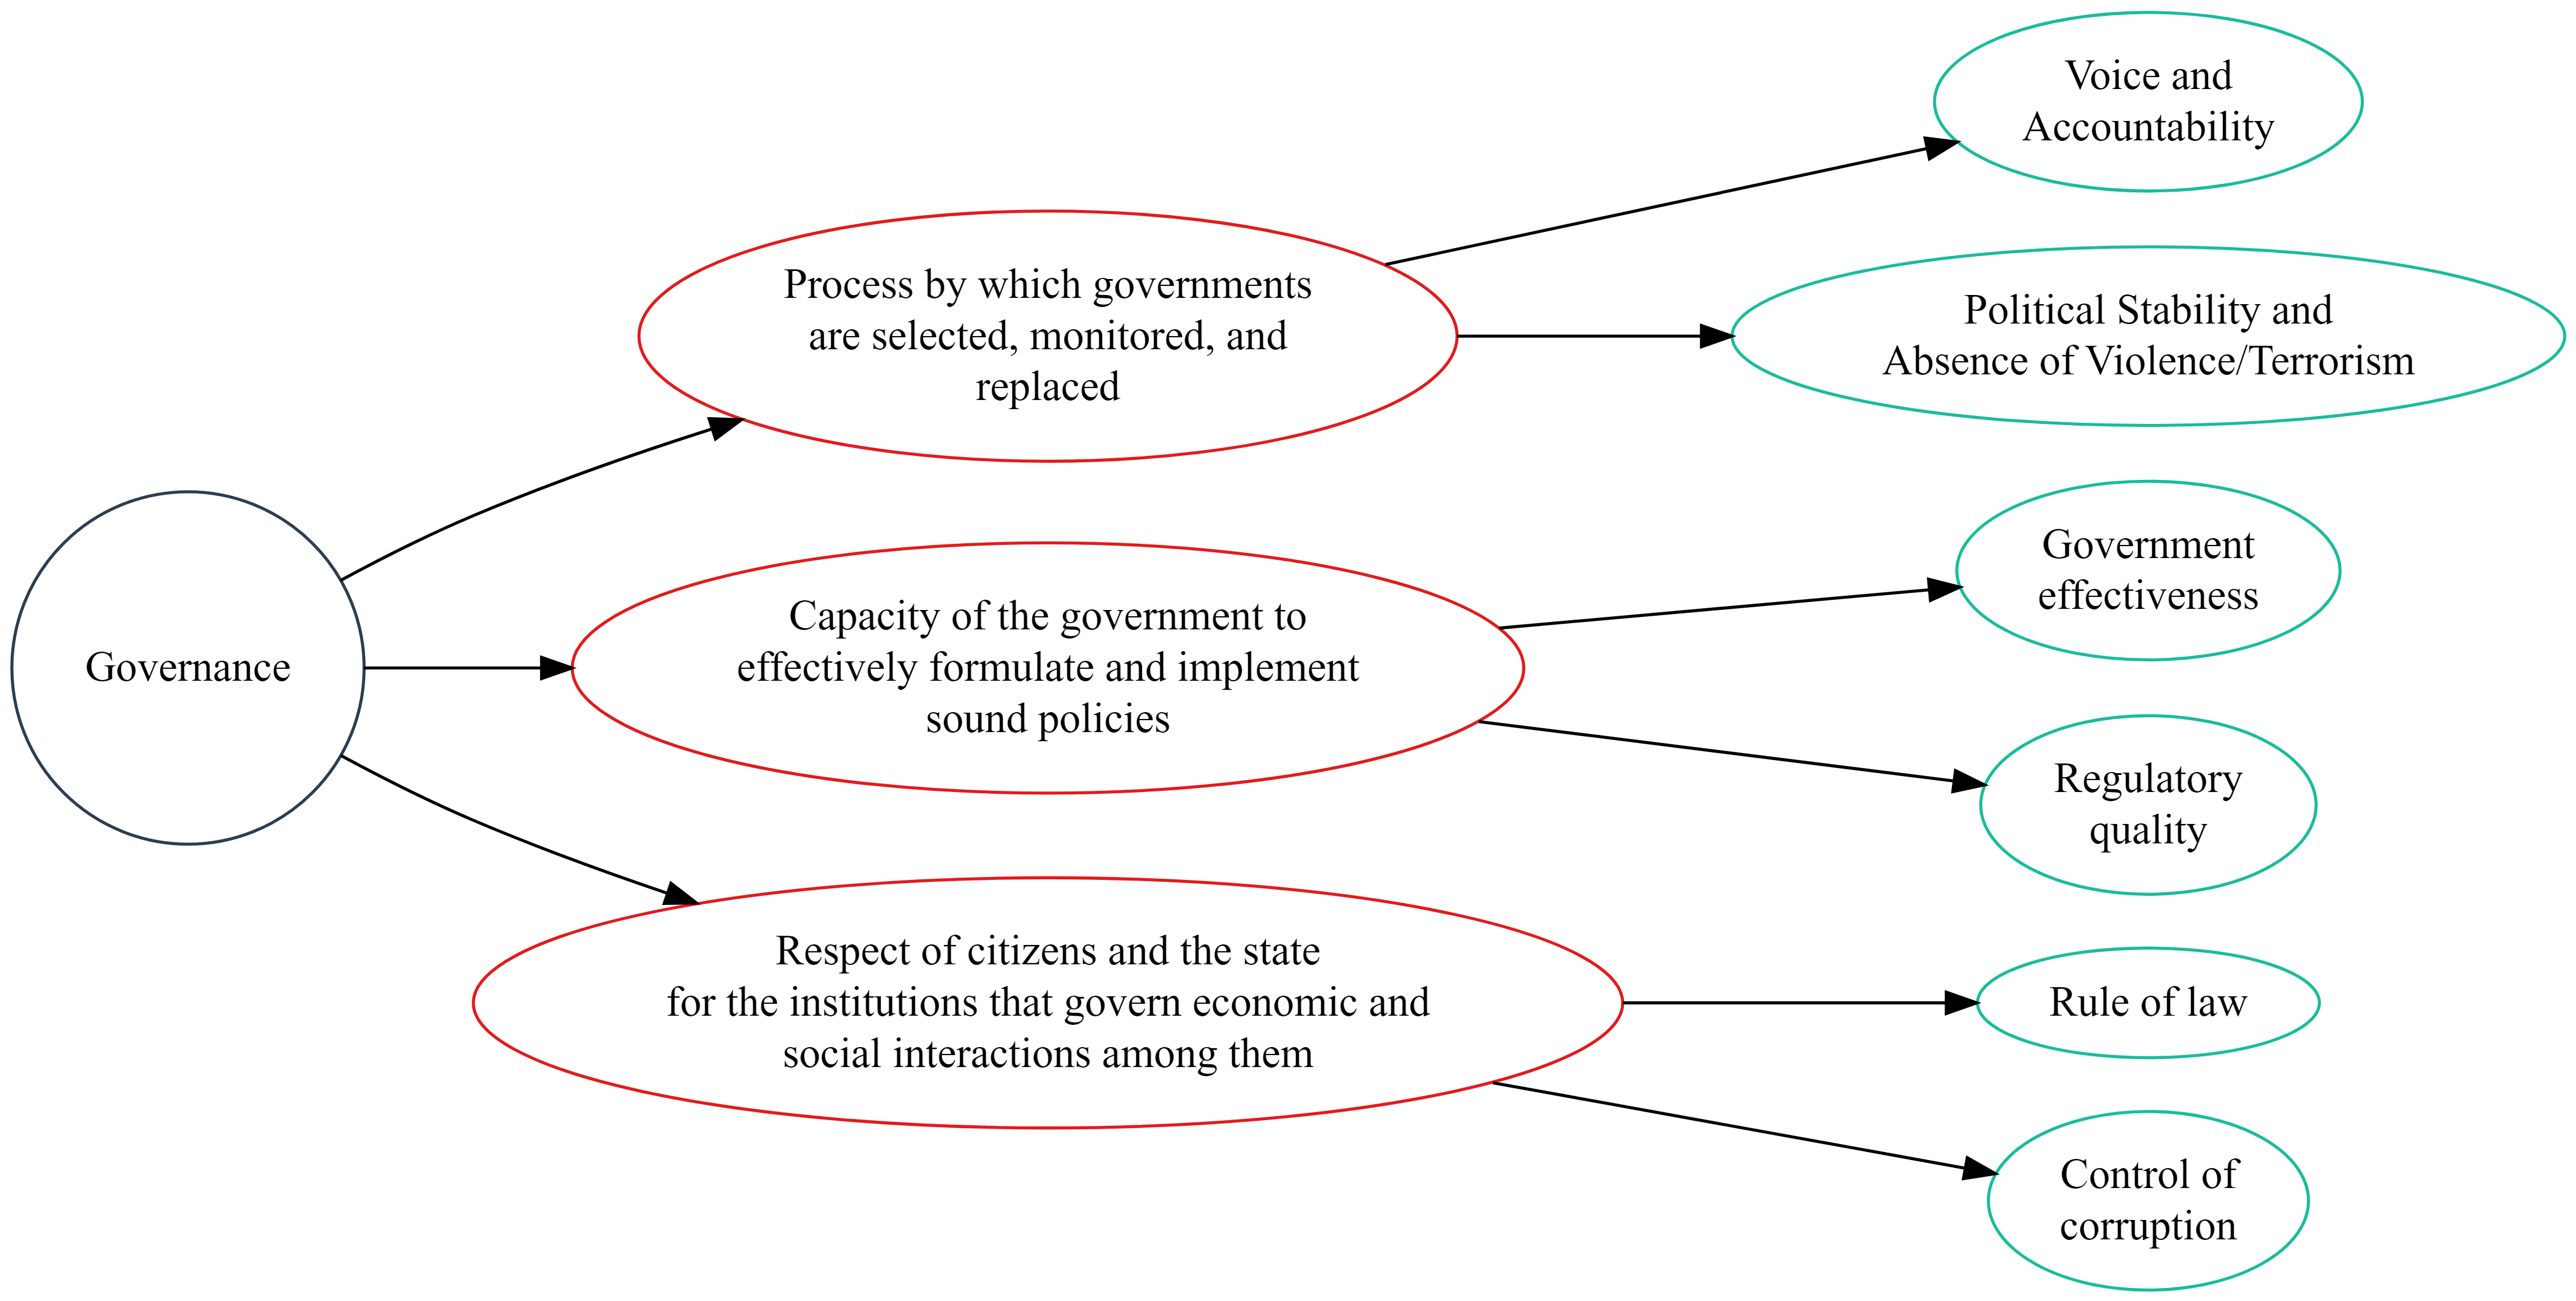
\includegraphics[width=5in,height=2in]{004_economy_institutions_files/figure-beamer/dot-figure-1.png}

}

\caption{\label{fig-governance-indicators}Governance dimensions
(\citeproc{ref-kaufmann_worldwide_2011}{Kaufmann, Kraay, and Mastruzzi
2011, 223})}

\end{figure}%
\end{frame}

\begin{frame}{}
\phantomsection\label{section-5}
\begin{itemize}
\item
  Where can I find data?

  \begin{itemize}
  \item
    Worldwide Governance Indicators (WGI) - WorldBank

    \begin{itemize}
    \tightlist
    \item
      \url{https://databank.worldbank.org/source/worldwide-governance-indicators}
    \end{itemize}
  \end{itemize}
\item
  What is the methodology?

  \begin{itemize}
  \tightlist
  \item
    \url{https://info.worldbank.org/governance/wgi/} \textgreater{}
    Documentation
  \end{itemize}
\end{itemize}
\end{frame}

\begin{frame}{}
\phantomsection\label{section-6}
\begin{figure}

\centering{

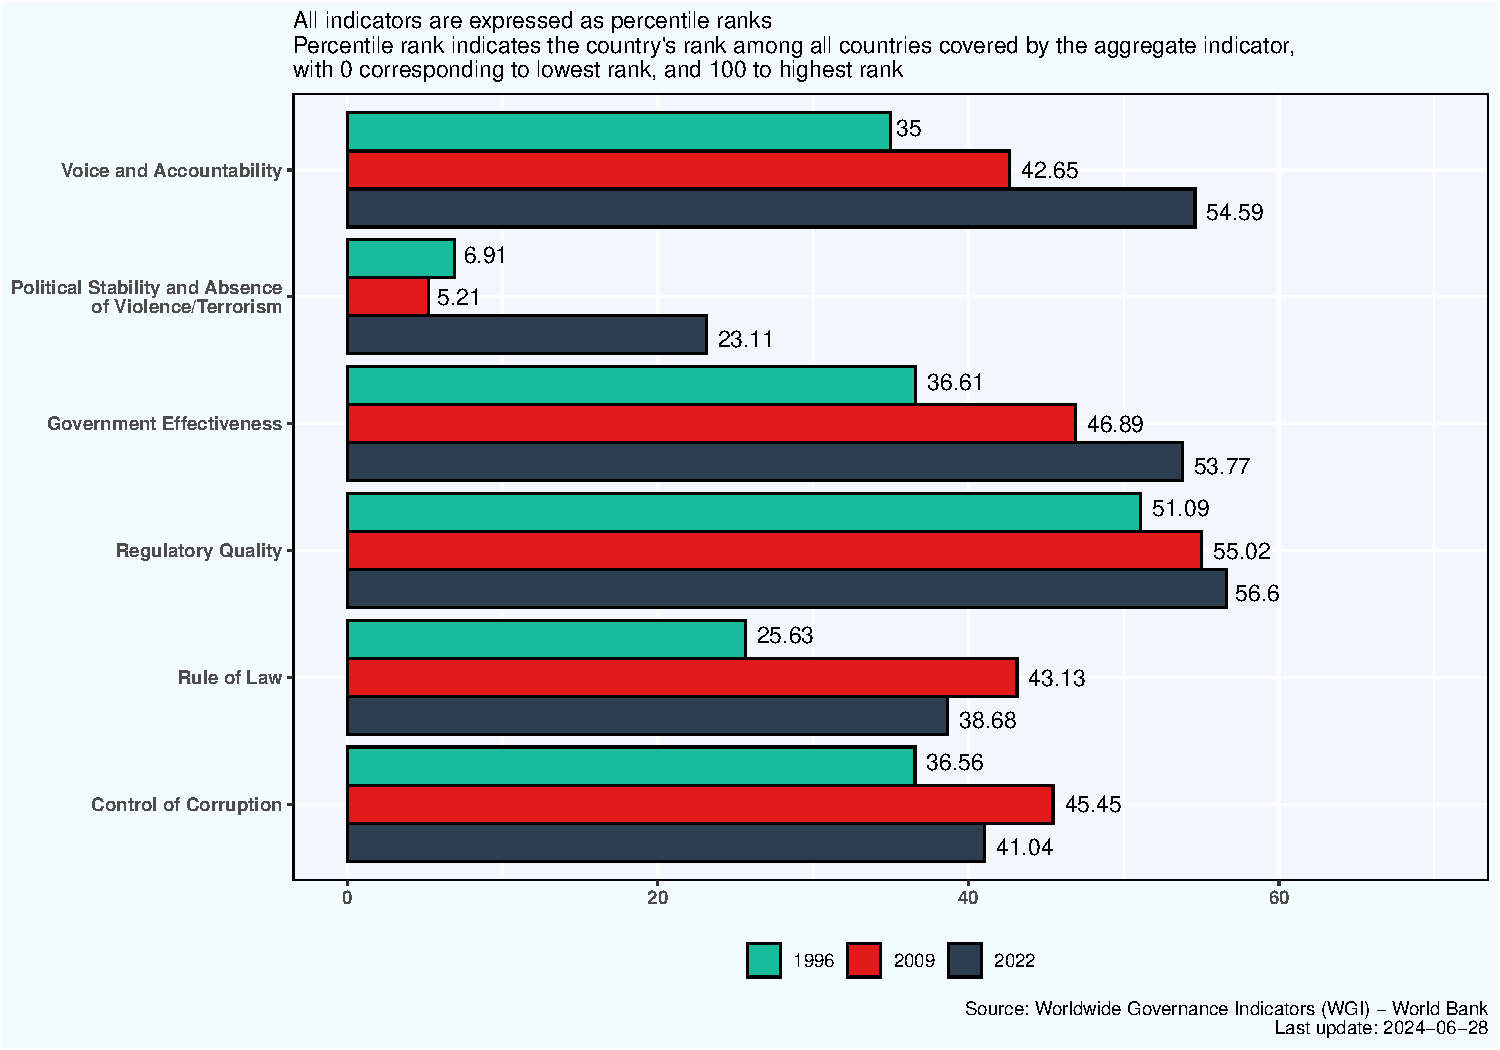
\includegraphics[width=0.85\textwidth,height=\textheight]{004_economy_institutions_files/figure-beamer/fig-governance-dimensions-col-1.pdf}

}

\caption{\label{fig-governance-dimensions-col}Governance dimensions for
Colombia}

\end{figure}%
\end{frame}

\section{Crime}\label{crime}

\begin{frame}{}
\phantomsection\label{section-7}
\begin{figure}

\centering{

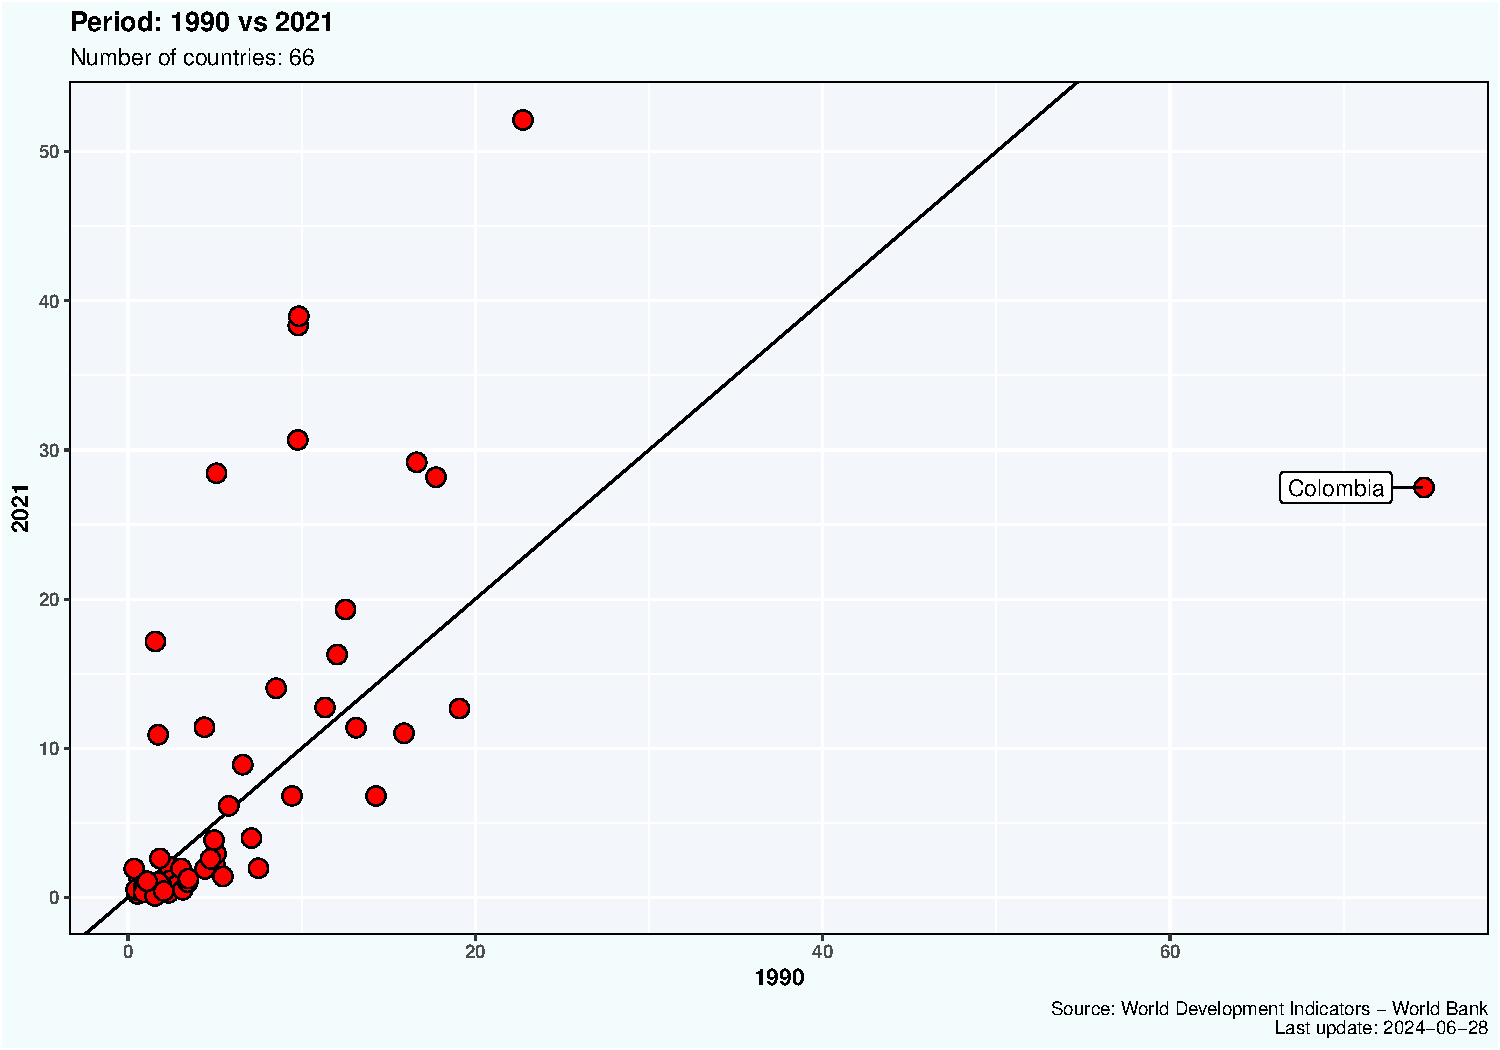
\includegraphics[width=0.85\textwidth,height=\textheight]{004_economy_institutions_files/figure-beamer/fig-intentional-homicides-col-1.pdf}

}

\caption{\label{fig-intentional-homicides-col}Intentional homicides (per
100,000 people)}

\end{figure}%
\end{frame}

\begin{frame}{}
\phantomsection\label{section-8}
\begin{figure}

\centering{

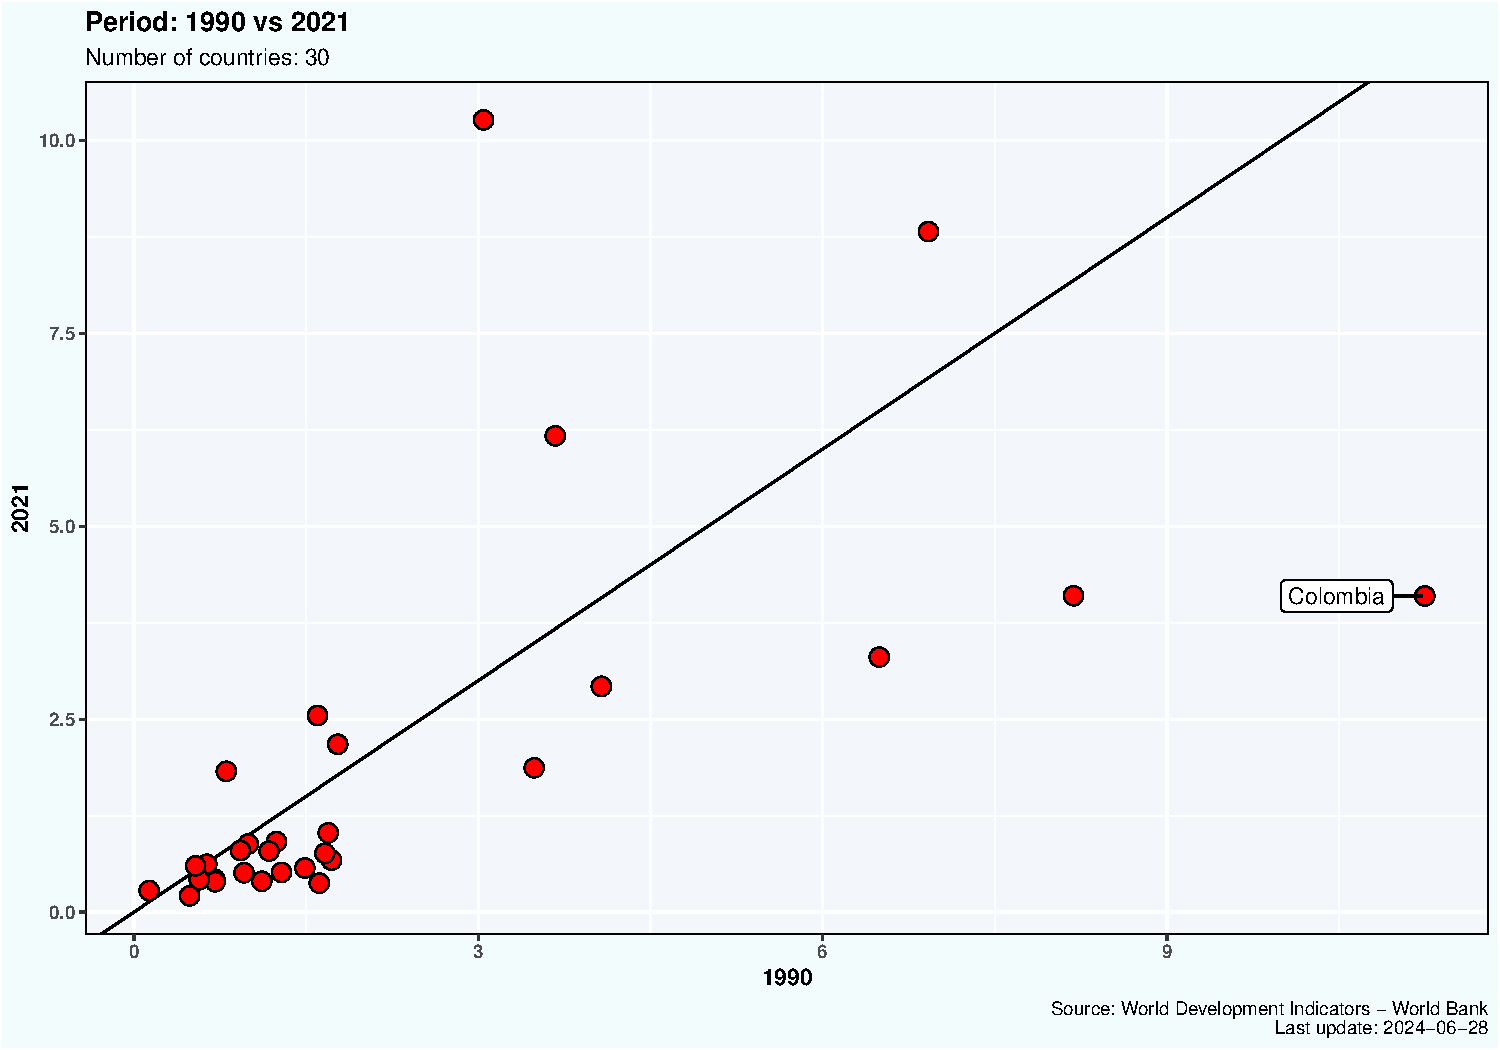
\includegraphics[width=0.85\textwidth,height=\textheight]{004_economy_institutions_files/figure-beamer/fig-intentional-homicides-female-col-1.pdf}

}

\caption{\label{fig-intentional-homicides-female-col}Intentional
homicides, female (per 100,000 female)}

\end{figure}%
\end{frame}

\begin{frame}{}
\phantomsection\label{section-9}
\begin{figure}

\centering{

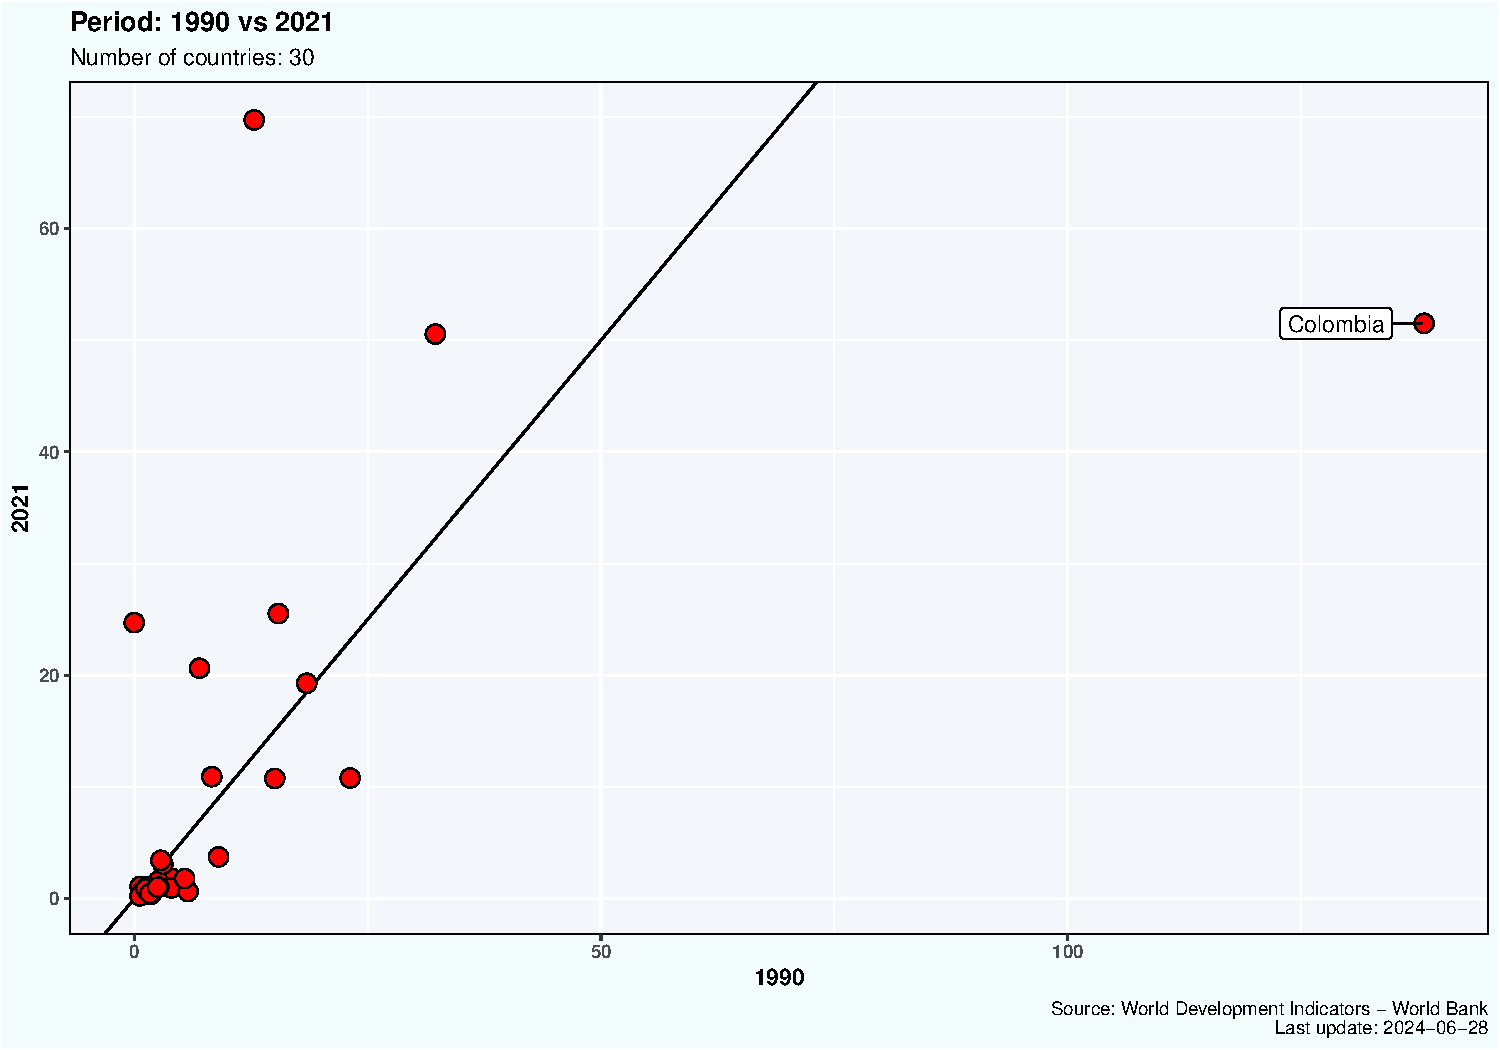
\includegraphics[width=0.85\textwidth,height=\textheight]{004_economy_institutions_files/figure-beamer/fig-intentional-homicides-male-col-1.pdf}

}

\caption{\label{fig-intentional-homicides-male-col}Intentional
homicides, male (per 100,000 male)}

\end{figure}%
\end{frame}

\begin{frame}{}
\phantomsection\label{section-10}
\begin{figure}

\centering{

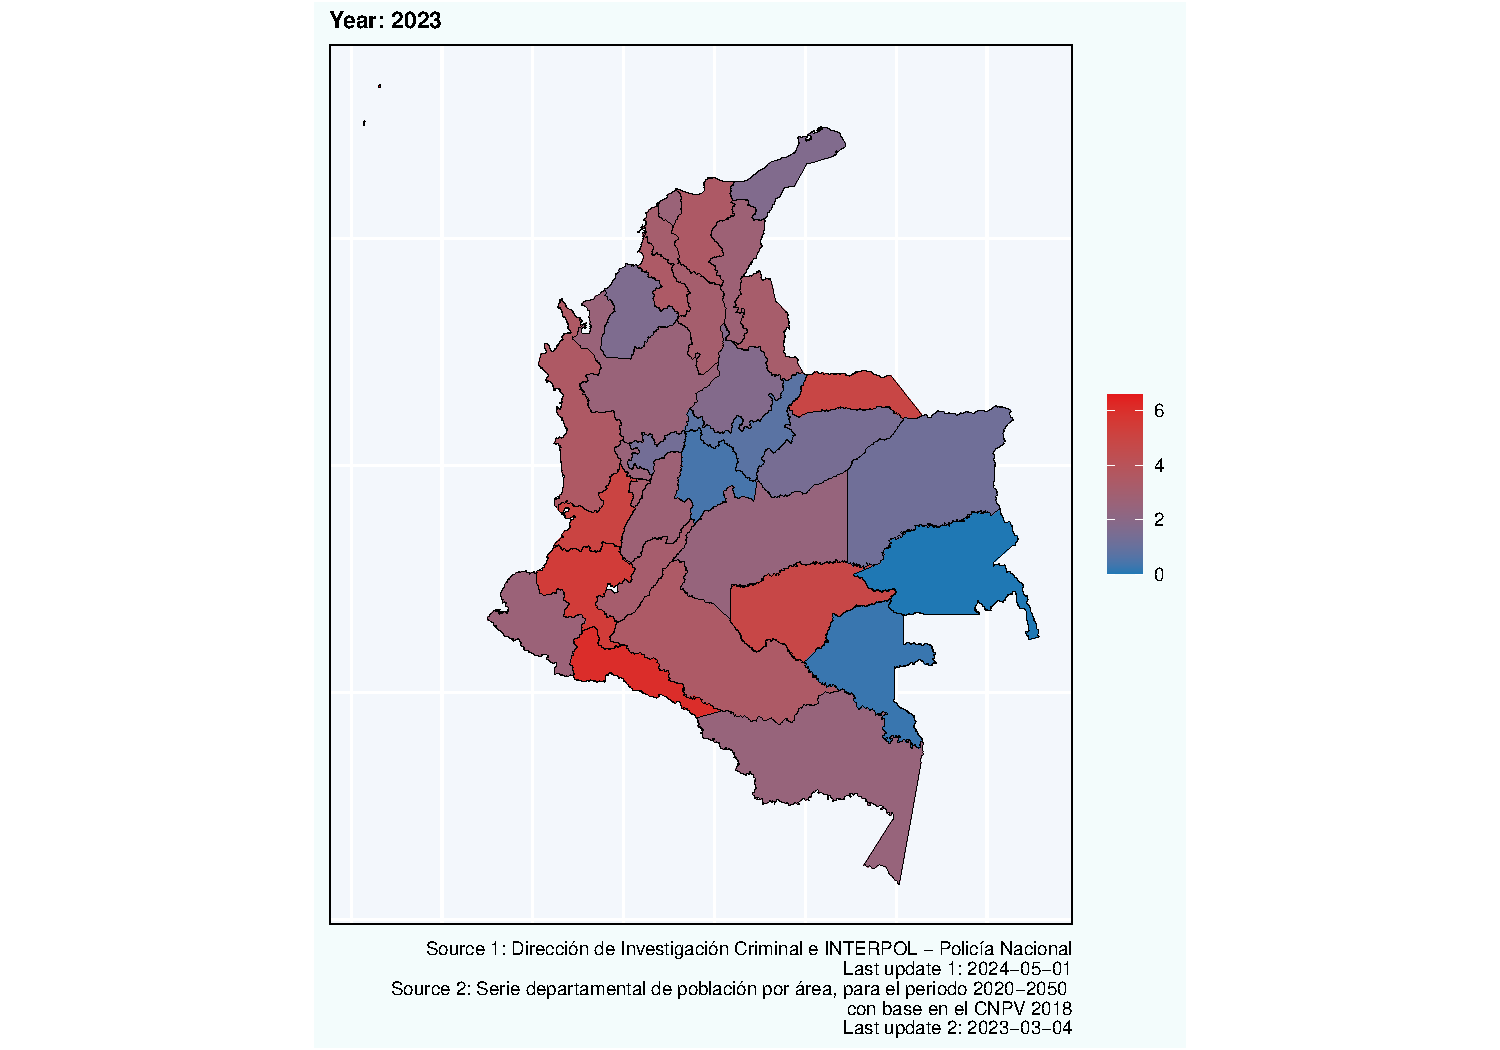
\includegraphics[width=0.85\textwidth,height=\textheight]{004_economy_institutions_files/figure-beamer/fig-map-homicides-col-1.pdf}

}

\caption{\label{fig-map-homicides-col}Intentional homicides (per 100,000
people) by department}

\end{figure}%
\end{frame}

\begin{frame}{}
\phantomsection\label{section-11}
\begin{figure}

\centering{

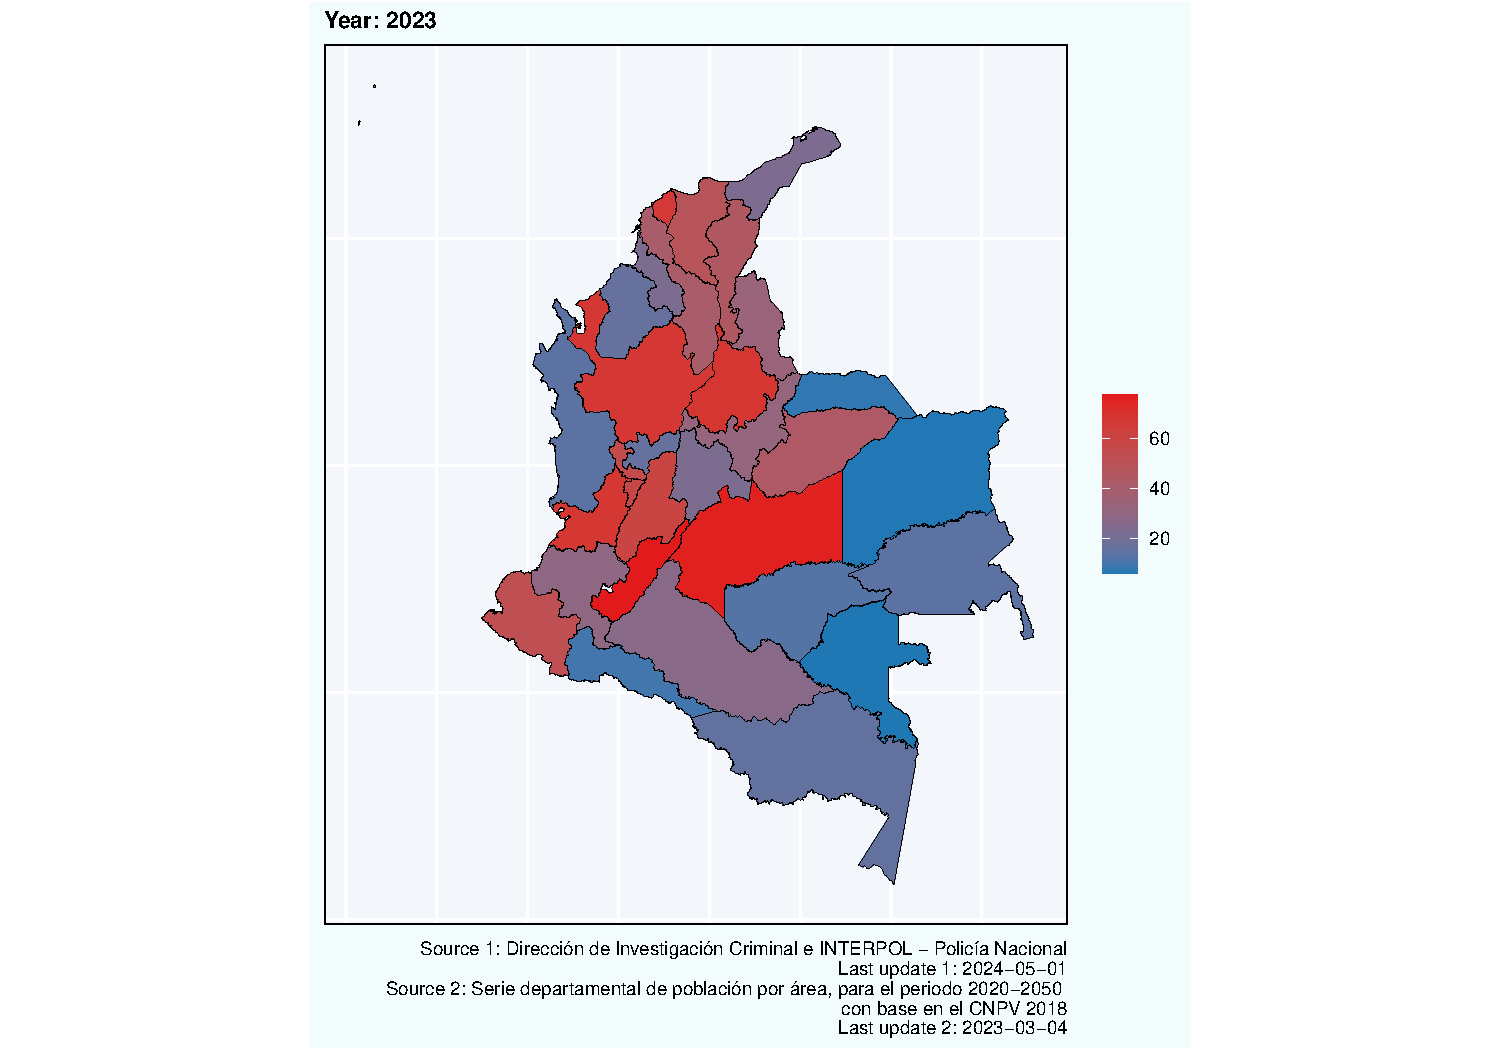
\includegraphics[width=0.85\textwidth,height=\textheight]{004_economy_institutions_files/figure-beamer/fig-map-theft-from-person-col-1.pdf}

}

\caption{\label{fig-map-theft-from-person-col}Theft from
person\footnote<.->{\emph{Hurto a personas} in spanish} (per 100,000
people) by department}

\end{figure}%
\end{frame}

\begin{frame}{}
\phantomsection\label{section-12}
\begin{figure}

\centering{

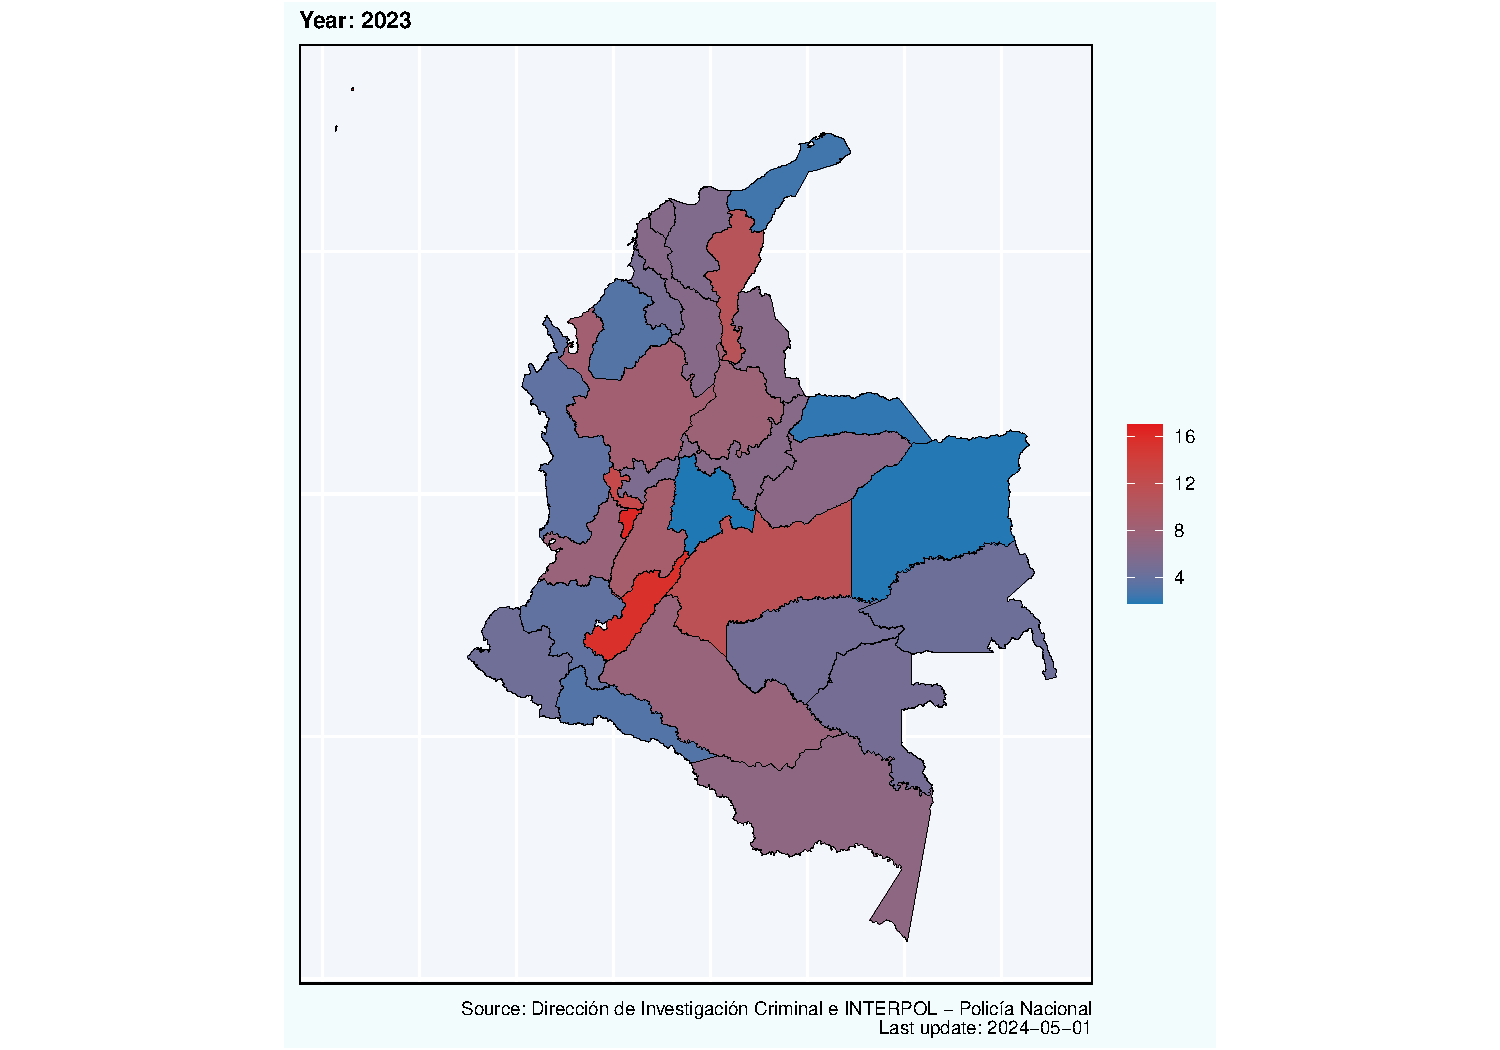
\includegraphics[width=0.85\textwidth,height=\textheight]{004_economy_institutions_files/figure-beamer/fig-map-theft-from-commercial-establishments-col-1.pdf}

}

\caption{\label{fig-map-theft-from-commercial-establishments-col}Theft
from commercial establishments\footnote<.->{\emph{Hurto a comercio} in
  spanish} (per 100,000 people) by department}

\end{figure}%
\end{frame}

\begin{frame}{}
\phantomsection\label{section-13}
\begin{figure}

\centering{

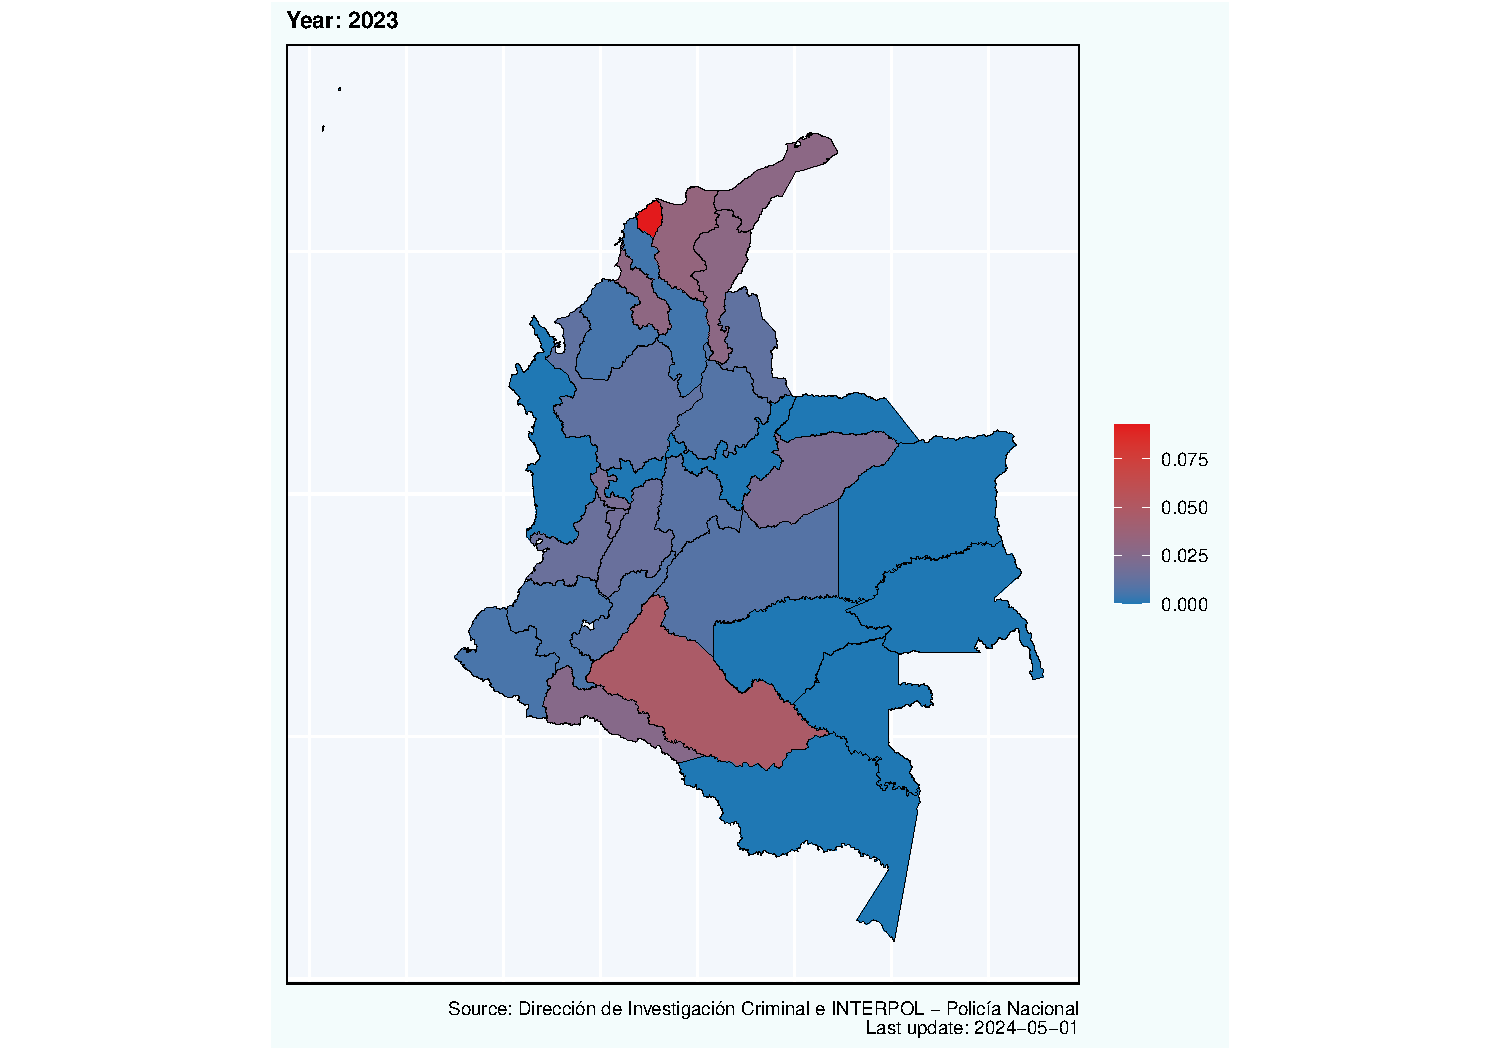
\includegraphics[width=0.85\textwidth,height=\textheight]{004_economy_institutions_files/figure-beamer/fig-map-robbery-financial-institutions-col-1.pdf}

}

\caption{\label{fig-map-robbery-financial-institutions-col}Robbery of
Financial Institutions\footnote<.->{\emph{Hurto a entidades financieras}
  in spanish} (per 100,000 people) by department}

\end{figure}%
\end{frame}

\begin{frame}{}
\phantomsection\label{section-14}
\begin{figure}

\centering{

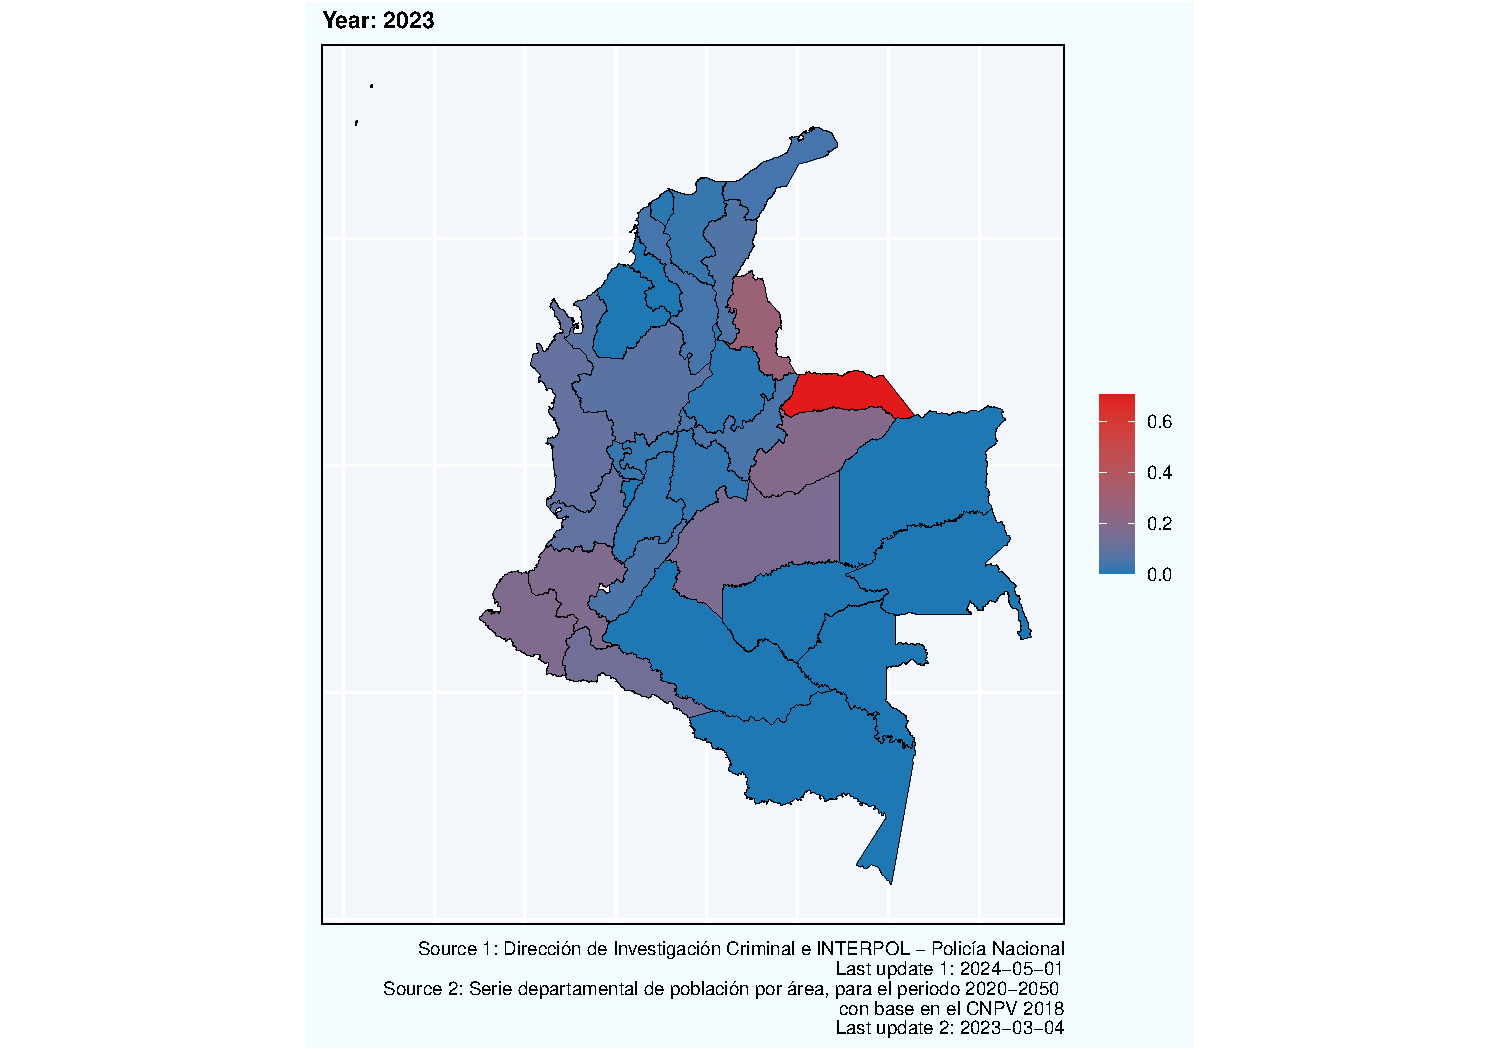
\includegraphics[width=0.85\textwidth,height=\textheight]{004_economy_institutions_files/figure-beamer/fig-map-kidnapping-col-1.pdf}

}

\caption{\label{fig-map-kidnapping-col}Kidnapping (per 100,000 people)
by department}

\end{figure}%
\end{frame}

\section{Acknowledgments}\label{acknowledgments}

\begin{frame}{}
\phantomsection\label{section-15}
\begin{itemize}
\item
  To my family that supports me
\item
  To the taxpayers of Colombia and the
  \href{https://www.umng.edu.co/estudiante}{\textbf{UMNG students}} who
  pay my salary
\item
  To the \href{https://www.business-science.io/}{\textbf{Business
  Science}} and \href{https://www.rfordatasci.com/}{\textbf{R4DS Online
  Learning}} communities where I learn
  \href{https://www.r-project.org/about.html}{\textbf{R}} and
  \href{https://www.python.org/about/}{\textbf{\(\pi\)-thon}}
\item
  To the \href{https://www.r-project.org/contributors.html}{\textbf{R
  Core Team}}, the creators of
  \href{https://rstudio.com/products/rstudio/}{\textbf{RStudio IDE}},
  \href{https://quarto.org/}{\textbf{Quarto}} and the authors and
  maintainers of the packages
  \href{https://CRAN.R-project.org/package=tidyverse}{\textbf{tidyverse}},
  \href{https://CRAN.R-project.org/package=wbstats}{\textbf{wbstats}},
  \href{https://CRAN.R-project.org/package=tidyquant}{\textbf{tidyquant}},
  \href{https://CRAN.R-project.org/package=janitor}{\textbf{janitor}},
  \href{https://CRAN.R-project.org/package=ggrepel}{\textbf{ggrepel}},
  \href{https://CRAN.R-project.org/package=sf}{\textbf{sf}} and
  \href{https://CRAN.R-project.org/package=tinytex}{\textbf{tinytex}}
  for allowing me to access these tools without paying for a license
\item
  To the \href{https://www.kernel.org/category/about.html}{\textbf{Linux
  kernel community}} for allowing me the possibility to use some
  \href{https://static.lwn.net/Distributions/}{\textbf{Linux
  distributions}} as my main
  \href{https://en.wikipedia.org/wiki/Operating_system}{\textbf{OS}}
  without paying for a license
\end{itemize}
\end{frame}

\section*{References}\label{references}
\addcontentsline{toc}{section}{References}

\begin{frame}[allowframebreaks]{References}
\phantomsection\label{refs}
\begin{CSLReferences}{1}{0}
\bibitem[\citeproctext]{ref-cardenas_introduccion_2020}
Cardenas, Mauricio. 2020. \emph{Introducción a La {Economía}
{Colombiana}}. 4th ed. Alfaomega.

\bibitem[\citeproctext]{ref-kaufmann_worldwide_2011}
Kaufmann, Daniel, Aart Kraay, and Massimo Mastruzzi. 2011. {``The
{Worldwide} {Governance} {Indicators}: {Methodology} and {Analytical}
{Issues}.''} \emph{Hague Journal on the Rule of Law} 3 (02): 220--46.
\url{https://doi.org/10.1017/S1876404511200046}.

\bibitem[\citeproctext]{ref-north_institutions_1991}
North, Douglass C. 1991. {``Institutions.''} \emph{Journal of Economic
Perspectives} 5 (1): 97--112. \url{https://doi.org/10.1257/jep.5.1.97}.

\bibitem[\citeproctext]{ref-north_institutions_1990}
North, Douglass C. 1990. \emph{Institutions, Institutional Change, and
Economic Performance}. The {Political} Economy of Institutions and
Decisions. Cambridge ; New York: Cambridge University Press.

\end{CSLReferences}
\end{frame}




\end{document}
